\documentclass[a4paper,10pt]{article}
\usepackage[utf8]{inputenc}
\usepackage[frenchb]{babel}
\usepackage{graphicx}
\renewcommand*\thesection{\arabic{section}}

%opening
\title{Resolution de problème - Problème des N-Reines}
\author{Jean-Baptiste Dalle}
\date{\today}

\begin{document}

\maketitle

\newpage

\tableofcontents

\newpage

\begin{abstract}

Résumé

\end{abstract}

\section{Introduction}

\section{Structure de données}

\section{Recherche locale}

\subsection{Implementation}

\subsection{Optimisation}

\section{Programmation par contrainte}

\subsection{Back Tracking}

\subsection{Forward Checking}

\subsection{Arc Consistancy 3}

\subsection{Heuristique}

\subsubsection{First find}

\subsubsection{Minimimum first}

\subsubsection{Maximum first}

\subsubsection{Random}

\subsubsection{Minimum domain size first}

\subsection{Performance}

\section{Conclusion}

\section{Annexe}

\subsection{Annexe 1 - Performance : Recherche locale}
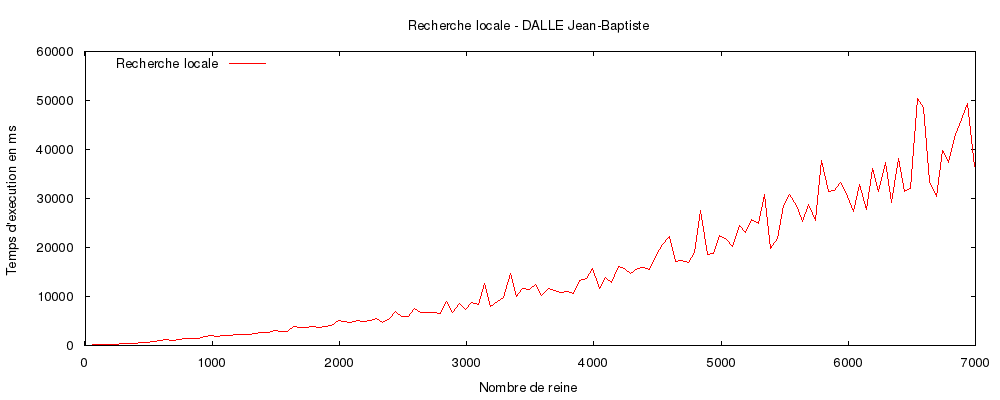
\includegraphics[width=1\textwidth]{Recherche_Locale.png}

\subsection{Annexe 2 - Performance : Programmation par contraintes}
\subsection{Annexe 3 - Performance : Programmation par contraintes - Back Tracking}
\subsection{Annexe 4 - Performance : Programmation par contraintes - Forward Checking}
\subsection{Annexe 5 - Performance : Programmation par contraintes - Random et Minimum domaine size}
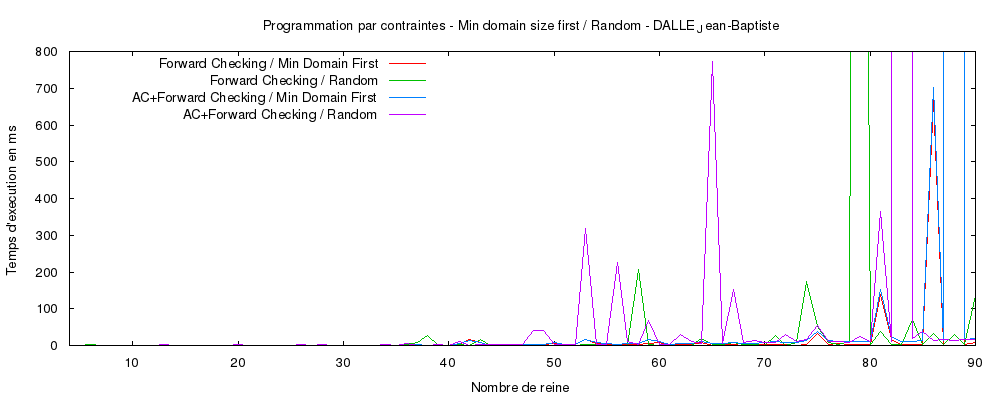
\includegraphics[width=1\textwidth]{Programmation_par_contraintes_-_Random_Min_Domain_Size.png}
\end{document}